\section{Technique}
\label{sec:technique}

We first give a high-level formulation of the problem (Section~\ref{sec:probl}), then present
the error detection algorithm (Section~\ref{sec:algorithm}). Finally, we show how to 
construct a reflection-aware call graph (Section~\ref{sec:cgcon}) and filter the error reports (Section~\ref{sec:heuristic}).


\subsection{Problem Formulation}
\label{sec:probl}

This section formulates the problem. We first define 
\textit{UI thread}, \textit{non-UI threads},
\textit{UI-accessing methods},
 \textit{safe UI methods}, and \textit{invalid thread access error}, and
state two assumptions we make with regard to error detection.

\vspace{1mm}
\noindent {\textsc{\textbf{Definition 1 (UI Thread).}}} {The UI thread
is a special thread created by the GUI framework during
GUI initialization. After the GUI becomes visible, the UI thread
takes charge of the application to handle events from the GUI\@.
It spawns new threads to process lengthy operations in the background. }
\vspace{1mm}

\noindent {\textsc{\textbf{Assumption 1.}}} {We assume that each multithreaded
GUI application has a single UI thread. This is true for applications
built on top of GUI frameworks adopting the single-GUI-thread rule. The
only exception is that 
 an application may fork a new process to launch another
application with its own UI thread. In that case, we require the
launched application to be analyzed separately.}\vspace{1mm}

\noindent {\textsc{\textbf{Definition 2 (non-UI Thread).}}} {Any other
threads except for the UI thread in a multithreaded GUI application
 are called non-UI threads.}\vspace{1mm}

\noindent {\textsc{\textbf{Assumption 2.}}} { We assume that each non-UI
thread is (transitively) spawned by the UI thread. Under this assumption,
we ignore all non-UI threads created by the GUI framework
before the UI thread has been initialized. That is, we assume all post-initialization
GUI work occurs in the UI thread. Once the GUI is visible, the
application is driven by events, which are always handled in the UI thread.
We believe this assumption is reasonable, since if a non-UI thread 
spawned during pre-initialization GUI work accesses a GUI object, an exception becomes
immediately apparent and the whole application may abort even before the
GUI is visible. This is highly unlikely for fielded GUI
applications.
}\vspace{1mm}

\noindent {\textsc{\textbf{Definition 3 (UI-Accessing Method).}}} { A method
whose execution may read or write a UI object is called a UI-accessing method.}\vspace{1mm}

\noindent  {\textsc{\textbf{Definition 4 (Safe UI Method).}}} {GUI frameworks that
adopt the single-GUI-thread rule must provide methods to permit non-UI threads
to run code in the UI thread, typically by sending a message to the UI thread.
We call such methods \textit{safe UI methods}, since
they can be invoked safely by any thread.}\vspace{1mm}

\noindent  {\textsc{\textbf{Definition 5 (Invalid Thread Access).}}} {An invalid-thread-access error results when the UI thread may spawn a non-UI thread, and there
exists a path from the non-UI thread's \CodeIn{start} method to any UI-accessing method
without going through any safe UI method. }\vspace{1mm}


\noindent  {\textsc{\textbf{Problem.}}}
At a high level, to detect an invalid thread access error, an analysis needs to track all
non-UI threads spawned by the UI thread, and check whether those non-UI threads
may invoke a UI-accessing method.\vspace{1mm}


\noindent  {\textsc{\textbf{Example.}}} Figure~\ref{fig:simplecg} shows an example call graph
to illustrate the invalid thread access problem.


\begin{figure}[t]
  \centering
  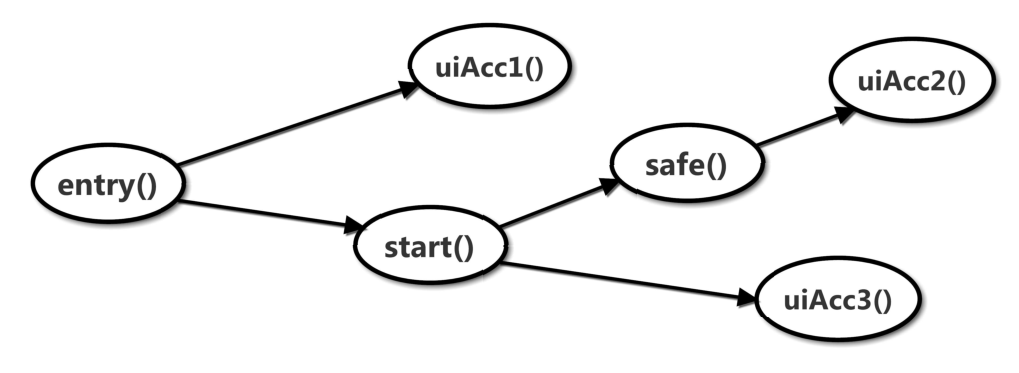
\includegraphics[scale=0.40]{simplecg-no-mark}
  \vspace*{-1.0ex}\caption {{\label{fig:simplecg} A simple call graph to illustrate the
invalid thread access problem. The \CodeIn{entry} method is executed
in a UI thread. Nodes \CodeIn{uiAcc1}, \CodeIn{uiAcc2}, and \CodeIn{uiAcc3} are
three UI-accessing methods. Node \CodeIn{safe} is a safe UI Method, and
node \CodeIn{start} is a (non-UI) thread-spawning method. Methods \CodeIn{uiAcc1}
and \CodeIn{uiAcc2} are executed in the UI thread, but method \CodeIn{uiAcc3}
is executed in a non-UI thread, causing an invalid thread access error.}}
\vspace{-2mm}
\end{figure}


\subsection{Error Detection Algorithm}
\label{sec:algorithm}

Figure~\ref{fig:detectalgorithm} shows the algorithm for detecting
potential invalid thread access errors. Our algorithm uses a
static call graph as the program representation for a multithreaded
GUI application. A Java call graph represents calling relationships
between methods. Specifically, each node represents a method and each
edge ($f$, $g$) indicates that method $f$ may call method $g$.
A theoretically ideal call graph is the union of the
dynamic call graphs over all possible executions of the program. 
A conservative, or sound, static call graph is a superset of
the ideal call graph; it over-approximates the
dynamic call graph of every possible execution. 
Because it is 
based on the call graph, our algorithm's reports are in terms of methods, as shown in Figure~\ref{fig:report}.

%In an object-oriented programming language like
%Java, a method is the basic logic unit in a program. Reporting
%potential errors at the method level can be sufficient in most cases.
%Thus, we believe using the call graph is well suited for this problem while
%compared with other program representations like control flow graph or
%program dependence graph. 


Our algorithm in Figure~\ref{fig:detectalgorithm} %works as follows. It
first constructs a static call graph for the tested program (line 2),
then specifies entry nodes, UI-accessing nodes, and safe UI nodes
for it on lines 3, 4, and 5, respectively. Lines 3--5 are GUI-framework-specific.
As an example, for a SWT desktop application, the entry nodes include
the single main method, UI-accessing nodes include methods
\CodeIn{Widget.checkWidget} and \CodeIn{Display.}\CodeIn{checkDevice},
and safe UI methods include two SWT helper methods \CodeIn{Display.asyncExec}  and
\CodeIn{Display.syncExec} for message passing. Section~\ref{sec:platforms}
explains the detailed instantiation for each supported framework.

The algorithm first performs graph traversal to find
all reachable \CodeIn{Thread.start()}
nodes from each entry node (line 7).
%For each entry node, the algorithm uses standard Breadth First Search (BFS)
%to find all reachable \CodeIn{Thread.start()} nodes (line 7).
Each \CodeIn{Thread.start()} node in a call graph indicates that a new,
non-UI thread is spawned.  The \CodeIn{Thread.start()}
nodes act as the sources in the main graph traversal.
The algorithm uses Breadth-First Search (BFS) to search for reachable UI-accessing
methods (lines 9--23).
The algorithm stops the traversal if it reaches a UI-accessing
method (lines 15--17) or a safe UI method (lines 18, 19).
%Specifically, it uses a queue to keep track of the nodes to be visited (line 7),
%and stores all visited nodes to avoid infinite loop (line 8).
%The algorithm checks every successive node to be visited (line 16):
%it reports an error if that node is a UI-accessing method (lines 18, 19), or skips
%it if it is a safe UI method (lines 20, 21), or simply keeps traversing otherwise (line 23).

The error message created by the method \CodeIn{createErrorReport} on line 16
includes the method call chain from the entry node to the UI-accessing node
as the error report. For brevity, the algorithm does not show the data structures that store
the current call chain.
The error report in Figure~\ref{fig:report} displays a method call chain from the entry
node \CodeIn{LayerView.<init>} to the UI-accessing node \CodeIn{ViewRoot}.\CodeIn{checkThread}.
%Note that when the algorithm determines that a UI-accessing method may be invoked
%by a non-UI thread, it computes a method call chain from the entry node to
%the UI-accessing node as the error report.
% does that. 



\begin{figure}[t]
\textbf{Input}: a Java program $\mathit{P}$\\
\textbf{Output}: a set of potential invalid thread access errors\\
%\textbf{Auxiliary Methods:}\\
%getSuccNodes($\mathit{g}$, $\mathit{n}$): return node $\mathit{n}$'s successive
%nodes in the graph $\mathit{g}$\\
\vspace{-4mm}
\begin{algorithmic}[1]
\STATE $\mathit{errors}$ $\leftarrow$ $\emptyset$ 
\STATE $\mathit{cg}$ $\leftarrow$ constructCallGraph($\mathit{P}$)
\STATE $\mathit{entryNodes}$ $\leftarrow$ getEntryNodes($\mathit{cg}$)
\STATE $\mathit{uiAccessingNodes}$ $\leftarrow$ getUIAccessingNodes($\mathit{cg}$)
\STATE $\mathit{safeUINodes}$ $\leftarrow$ getSafeUINodes($\mathit{cg}$)\\
\FOR{each $\mathit{entryNode}$ in $\mathit{entryNodes}$}
\STATE $\mathit{worklist}$ $\leftarrow$ getReachableStarts($\mathit{entryNode}$)
\STATE $\mathit{visited}$ $\leftarrow$ $\emptyset$
\WHILE{$\mathit{worklist}$ $\neq$ $\emptyset$}
\STATE $\mathit{node}$ $\leftarrow$ $\mathit{worklist}$.dequeue()
\IF{$\mathit{node}$ $\in$ $\mathit{visited}$}
\STATE continue
\ENDIF
\STATE $\mathit{visited}$ $\leftarrow$ $\mathit{visited}$ $\cup$ $\mathit{node}$
\IF{$\mathit{node}$ $\in$ $\mathit{uiAccessingNodes}$}
\STATE $\mathit{newError}$ $\leftarrow$ createErrorReport($\mathit{node}$)
\STATE $\mathit{errors}$ $\leftarrow$ $\mathit{errors}$ $\cup$ $\mathit{newError}$
\ELSIF{$\mathit{node}$ $\in$ $\mathit{safeUINodes}$}
\STATE continue
\ELSE
\STATE $\mathit{worklist}$.enqueueAll(getSuccNodes($\mathit{cg}$, $\mathit{node}$))
\ENDIF 
\ENDWHILE
\ENDFOR
\RETURN $errors$
%\ENDWHILE
\vspace{-2mm}
\end{algorithmic}
\caption{Algorithm for detecting invalid thread access errors in multithreaded GUI programs. 
Any call graph construction algorithm can be used (line 2). The algorithm
is parameterized by the three methods in lines 3--5 which are specific to each GUI framework
 as described in Section~\ref{sec:platforms}.
} \label{fig:detectalgorithm}
\end{figure}

The algorithm in Figure~\ref{fig:detectalgorithm} uses BFS to search
for potential error-revealing paths, since BFS always returns the
shortest path to the UI-accessing node, permitting
smaller error reports. However,
other graph search strategies such as Depth-First Search (DFS) or
exhaustive path search can also be employed. In our experiment (Section~\ref{sec:search}),
we empirically compared three different graph search strategies, and demonstrated that
using BFS, the algorithm found more errors than DFS and was more practical than
exhaustive path search.

\tinystep

\subsection{Call Graph Construction}
\label{sec:cgcon}

%Given a sound call graph, our algorithm is sound in that it does not
%miss true positives. We note, however, 
For some modern GUI applications, computing a good
call graph in the presence of reflection and native methods is non-trivial. 
To alleviate this problem, we next present a reflection-aware call graph
construction algorithm in Section~\ref{sec:cg} and annotation support
for native methods in Section~\ref{sec:annotation}.

\subsubsection{Reflection}
\label{sec:cg}

%In OO program, translate k-CFA as:
%k-call-site sensitive interprocedural pointer
%analysis with a k-context-sensitive heap and onthe-
%fly call-graph construction
% 

\begin{figure}[t]
%\centering
\begin{CodeOut}
\begin{alltt}
<LinearLayout>
    <Button android:id="@+id/\textbf{button\_id}" android:text="A Button" />
</LinearLayout>

1. public class MyActivity extends Activity \ttlcb
2.    @Override
3.    public void onCreate(Bundle savedInstanceState) \ttlcb
4.        super.onCreate(savedInstanceState);
5.        setContentView(R.layout.main);
6.        Button button = (Button) findViewById(R.id.\textbf{button\_id});
7.        button.setOnClickListener(new Button.OnClickListener() \ttlcb
8.            @Override
9.            public void onClick(View v) \ttlcb
10.               button.setText("Button Clicked.");
11.           \ttrcb
12.       \ttrcb);
13.   \ttrcb
14. \ttrcb
\end{alltt}
\end{CodeOut}
\vspace*{-3.0ex} \caption{Sample GUI application code on the Android platform. The layout
XML file (the top) specifies a Button object declaratively, 
and the Java code (the bottom)
first loads the XML file (line 5) and then uses reflection to create
a Button object by its ID (line 6, the \CodeIn{findViewById} method).}
\label{fig:sampleandroid}
\end{figure}



\begin{figure}[t]
\vspace{3mm}
\textbf{Input}: a Java program $\mathit{P}$\\
\textbf{Output}: a call graph $\mathit{cg}$\\
\vspace{-4mm}
\begin{algorithmic}[1]
\FOR{each $\mathit{expression}$ in $\mathit{P}$}
\IF{isReflectionCall($expression$)}
\STATE $\mathit{objectSet}$ $\leftarrow$ getAllObjectsThatMayBeCreated($\mathit{expression}$)
\STATE $\mathit{newExpr}$ $\leftarrow$ createObjectCreationExpression($\mathit{objectSet}$)
\STATE replace $\mathit{expression}$ with $\mathit{newExpr}$
\ENDIF
\ENDFOR
\STATE $\mathit{cg}$ $\leftarrow$ constructCallGraph($\mathit{P}$)
\RETURN $\mathit{cg}$
%\ENDWHILE
\end{algorithmic}
\vspace{-3mm}
\caption{A reflection-aware call graph construction algorithm. Lines
1--7 are a simple program transformation to replace reflection calls
with object creations, and line 8 builds the call graph using
an existing call graph construction algorithm. This algorithm
is parameterized by two methods on lines 2 and 3. 
How to instantiate it for the Android framework is presented in Section~\ref{sec:cg}.
} 
\label{fig:cgalgorithm}
\end{figure}

%GUI applications tend to use reflection intensively. In particular,
GUI applications built on top of the Android framework
use configuration files and reflection to specify GUI layout.
As a result, call graph construction algorithms such as RTA~\cite{rta}
and k-CFA~\cite{kcfa} fail to build a sufficiently complete call graph.
The example code in Figure~\ref{fig:sampleandroid} from an Android application
 illustrates the limitations.
In Figure~\ref{fig:sampleandroid}, line 6 uses reflection to create a \CodeIn{Button}
object by looking up its id declared in the associated XML file. When this button
is clicked, its event handling code (lines 9--11) updates the text.

When analyzing the code in Figure~\ref{fig:sampleandroid}, existing call graph algorithms
fail to conclude that the variable \CodeIn{button} declared on line 6
points to a \textit{non-null} \CodeIn{Button} object due to their limitations in handling the
reflection call \CodeIn{findViewById}. The resulting call graph
omits the edge corresponding to the \CodeIn{setText} method call on line 10.

To address this limitation, we present an algorithm to construct
a reflection-aware call graph based on a simple program transformation.
The basic idea is to replace reflection calls with explicit object
creation expressions, pretending that the corresponding concrete object
has been created.  The algorithm is shown in Figure~\ref{fig:cgalgorithm}.
It consists of two steps. The first step (lines 1--7) is a simple program
transformation to replace reflection calls with object creation expressions, and
the second step (line 8) uses an existing call graph construction algorithm
to build the graph on the transformed program. In our context,
a reflection call represents a framework-specific helper method invocation
that uses Java reflection to create desirable objects, such as
the \CodeIn{findViewById} method in Android applications, instead
of the methods in the \CodeIn{java.lang.reflection} package.
When it sees a reflection call, the algorithm
determines a set of possible objects that might be created.
After that, the algorithm creates an expression that non-deterministically
returns a new object from the object set.

This algorithm is parameterized by two methods on
lines 2 and 3. When instantiated for the Android framework,
the predicate isReflectionCall on line 2 returns true
if the $expression$ is a \CodeIn{findViewById(id)} method call, and the method
getAllObjectsThatMayBeCreated on line 3 parses the associated XML configuration
file to extract the class declaration
 corresponding to the given \CodeIn{id} value. If the \CodeIn{id}
value is dynamically generated, this method will conservatively
return instances of all subclasses of the declared type.
%On line 8, any existing call graph construction algorithm can be applied.

Take the code in Figure~\ref{fig:sampleandroid} as an example.
When the algorithm sees the reflection call
\CodeIn{findViewById(R.id.button\_id)}, it
parses the XML configuration file to determine that the \CodeIn{button\_id}
value is mapped to a \CodeIn{Button} instance. Then, it
replaces the reflection call
with an explicit object creation expression: \CodeIn{new Button(null)}.
After that, the algorithm employs existing call graph construction
algorithms to analyze the transformed program, and permits them
to include the call edge \CodeIn{setText} in the resulting graph.

As demonstrated in our experiments, this reflection-aware call
graph construction algorithm helps in detecting errors
in Android applications (Section~\ref{sec:reflectionaware}).


\subsubsection{Native Methods}
\label{sec:annotation}

A GUI application may use native methods to interact with the underlying
operating system or platform. Native methods are often
beyond the ability of a static analysis but should be considered to make
the call graph more complete. To do so, we provide an annotation \CodeIn{@CalledByNativeMethods}
for users to specify which native methods may call the current method. For example,
the following code snippet indicates that native methods \CodeIn{native1()} and \CodeIn{native2()}
may call method \CodeIn{javaMethod()}.

%\noindent 
\CodeIn{@CalledByNativeMethods(callers=\ttlcb"native1", "native2"\ttrcb)}

%\noindent
\CodeIn{public void javaMethod() \ttlcb\ ... \ttrcb}


\noindent Our static analysis takes the call relationship specified by this
annotation into consideration when traversing the call graph. 

Adding annotations for native methods is optional and requires manual effort.
In our experiments, 1 out of \subnum programs (SGTPuzzler) uses native methods. We manually
searched the Java source files to find all native methods,
inspected the C code to determine possible target methods
that may be called by a native method, and added \annotationnum annotations for this program.
We found such annotations were useful: one error
is only reported when using the user-provided annotations.


\subsection{Filtering the Error Reports}
\label{sec:heuristic}

A static analysis can check possible error paths without executing the
code, but it may report
paths that do not actually exist (false positives) or multiple paths
that have the same error cause (redundant warnings). We devised
5 error filters to remove likely false positives and redundant warnings.
The first 2 filters are sound in that they will not filter real bugs, and
the other 3 filters are based on heuristics. Orthogonally, filters 2
and 3 are for reducing false positives, and filters 1, 4, and 5
are for reducing redundant warnings.

%1 - subsumed, 2 - user annotated, 3 - sysem call, 4 heand  5,  tail


%To remove those 
%The potentially huge volume of
%reported warnings impose great burden for programmers to check
%its validity. 


%\begin{enumerate}

%\item

% \subsubsection{Sound Filters}

\textbf{1. Filter Lexically Redundant Reports}. One reported method call
chain can lexically subsume another one. For example, suppose that two
reported method call chains, \CodeIn{a()} $\rightarrow$ \CodeIn{b()}
$\rightarrow$ \CodeIn{c()} and 
\CodeIn{d()} $\rightarrow$ \CodeIn{a()} $\rightarrow$ \CodeIn{b()} $\rightarrow$ \CodeIn{c()},
both lead to a potential error, since $\CodeIn{d()}$ and \CodeIn{a()}
are two distinct entry methods. The second call chain can
be removed without missing any errors, since
the first chain reveals the same error and is shorter 
for programmers to interpret.


%\item
\textbf{2. Filter Reports with User-Annotated Methods}. Users are
permitted to explicitly annotate specific methods
that will never trigger an error.
%For example, the Android GUI framework provides a utility method 
%\CodeIn{runOnUIThread} to check whether the current thread is the UI thread
%before executing the code. If the current thread is not the UI thread,
%this method will be executed on the UI thread via message passing.
%Thus,
Assuming the user annotations are accurate,
a reported method call chain containing an annotated method
can be safely removed. 

In our experiments, 
we produced a list of \filternum annotated methods for two
subjects (MyTracks and Fennec), since they employ a customized pattern
to interact with the GUI framework. For example, in MyTracks, all non-UI
threads are initialized via using the library method \CodeIn{android.os\-.handler.handleCallback}.
This method can be invoked from any thread and will never cause an
invalid thread access error, because it checks whether the current
thread is the UI thread or not before execution. If not,
this method will use safe UI methods to run the code in the UI thread.




% we produced a list of \filternum
%annotated methods for two subjects (Fennec and MyTracks) because they use a customized
%pattern to interact with the GUI framework.



% \subsubsection{Heuristic Filters}
%\item

\textbf{3. Filter Reports Containing Library Calls}. A
method call chain containing certain library calls
like \CodeIn{Runtime.}\CodeIn{shutDown} are unlikely to
be buggy. For example, the \CodeIn{Runtime.}\CodeIn{shutDown}
method is called when the JVM terminates, and uses multithreading
to dispose all GUI objects when the program exits.
Our experiments use a list of \libnum such library calls.

\textbf{4. Filter Reports with the Same Head Methods from the Entry Node to \CodeIn{Thread.start()}}. A method can call
multiple methods that access GUI objects, such as:

\pagebreak[3]
\vspace{-2mm}                   %
\begin{CodeOut}
\begin{alltt}
     public void m() \ttlcb
         accessUIObject1();
         accessUIObject2();
     \ttrcb
\end{alltt}
\end{CodeOut}
\vspace{-2mm}
If method \CodeIn{m()} is invoked by a non-UI thread, our algorithm will
report method call chains that
only differ in the last few method nodes, such as:

\CodeIn{a()} $\rightarrow$ ...\CodeIn{Thread.start()} ... $\rightarrow$ \CodeIn{m()} $\rightarrow$ \CodeIn{accessUIObject1()} ...

\CodeIn{a()} $\rightarrow$ ...\CodeIn{Thread.start()} ... $\rightarrow$ \CodeIn{m()} $\rightarrow$ \CodeIn{accessUIObject2()} ...

\noindent
These two chains may have the same error root cause: knowing that
method \CodeIn{m()} is called by a non-UI thread is sufficient to understand
the error.
This filter compares two reported chains that have the same
head methods from the entry node to \CodeIn{Thread}.\CodeIn{start()},
and removes the longer one.
%$k$ ($k$ is user-settable with a default value 5 as used in our
%experiments) head nodes, and removes the longer one.

%\item
\textbf{5. Filter Reports with the Same Tail Methods from \CodeIn{Thread}.
\CodeIn{start()}
to the UI-accessing Method}. A method
can have multiple callers, so method call chains with the same tail are likely
to just represent different ways to trigger the same error. This filter compares 
two reported method call chains that share the same 
tail from \CodeIn{Thread.start()} to the UI-accessing methods, and
removes the longer one. Using filters 4 and 5 together results in
only one error per \CodeIn{Thread.start()}.



%\end{enumerate}
\vspace{1mm}

In our experiments (Section~\ref{sec:filters}), these filters remove
99.96\% of the reported warnings.
We also found that using sound filters alone was insufficient, because an overwhelming
number of warnings remained.  This motivated our use
of heuristic filters.


%%% Local Variables: 
%%% mode: latex
%%% TeX-master: "guierror"
%%% TeX-command-default: "PDF"
%%% End: 

%  LocalWords:  multithreaded pre SWT checkWidget checkDevice asyncExec
%  LocalWords:  syncExec BFS createErrorReport LayerView init ViewRoot
%  LocalWords:  checkThread constructCallGraph getEntryNodes newError
%  LocalWords:  getUIAccessingNodes getSafeUINodes getReachableStarts
%  LocalWords:  uiAccessingNodes safeUINodes worklist objectSet newExpr
